\documentclass[10pt, aspectratio=169, handout]{beamer}
\usefonttheme{professionalfonts}

\mode<presentation>
{
  \usetheme{Berkeley}
  \usecolortheme{beaver}
  \usefonttheme{default}
  \setbeamertemplate{navigation symbols}{}
  \setbeamertemplate{caption}[numbered]
} 

\setbeamertemplate{footline}{%
  \leavevmode%
  \hbox{%
    \begin{beamercolorbox}[wd=.85\paperwidth,ht=2.5ex,dp=1ex,left]{author in head/foot}%
      \usebeamerfont{author in head/foot}Maxx Seminario, Electronic Circuits, Spring 2026%
    \end{beamercolorbox}%
    \begin{beamercolorbox}[wd=.15\paperwidth,ht=2.5ex,dp=1ex,right]{date in head/foot}%
      \hspace*{0.5em}\insertframenumber{} / \inserttotalframenumber\hspace*{0.5em}%
    \end{beamercolorbox}%
  }%
  \vskip0pt%
}

\usepackage[english]{babel}
\usepackage[utf8]{inputenc}
\usepackage{tikz}
\usepackage{pgfplots}
\usepackage{array}
\usepackage{makecell}
\usepackage{verbatim}
\usepackage{graphicx}
\usepackage{subcaption}
\usepackage{amsfonts}
\usepackage{amsmath}
\usepackage{bm}
\usepackage{epstopdf}
\usepackage[american]{circuitikz}
\usepackage{caption}
\captionsetup{compatibility=false}
\usepackage[absolute,overlay]{textpos}
\usetikzlibrary{calc}
\usetikzlibrary{pgfplots.fillbetween, backgrounds}
\usetikzlibrary{positioning}
\usetikzlibrary{pgfplots.groupplots}
\usetikzlibrary{plotmarks}
\usetikzlibrary{calc}
\usetikzlibrary{decorations.markings}
\usetikzlibrary{arrows.meta}

\usepgfplotslibrary{groupplots}
\pgfplotsset{compat=newest} 

\usepackage{hyperref}
\hypersetup{
    colorlinks=true,
    linkcolor=blue,
    filecolor=magenta,      
    urlcolor=cyan,
}

% Added by Maxx Seminario 01/06/2026 - for colored icons in itemize labels
\usepackage{wasysym} % for smiles and frowns
\newcommand{\neutralface}{%
  \tikz[baseline=-0.6ex]{
    \draw (0,0) circle (0.9ex);
    \fill (-0.35ex,0.25ex) circle (0.12ex);
    \fill ( 0.35ex,0.25ex) circle (0.12ex);
    \draw (-0.35ex,-0.25ex) -- (0.35ex,-0.25ex);
  }%
}

\newcommand{\baditem}{\textcolor{red!70!black}{\frownie}}
\newcommand{\gooditem}{\textcolor{green!60!black}{\smiley}}
\newcommand{\mehitem}{\textcolor{orange!80!black}{\neutralface}}


\title[ECEN 222]{Time Domain Analysis of RLC Circuits}
\author{Maxx Seminario}
\institute{University of Nebraska-Lincoln}
\date{Spring 2026}

\begin{document}
\begin{frame}
  \titlepage
\end{frame}

\section{Introduction to Time Domain Analysis}

\begin{frame}{Why Time Domain Analysis?}
    
    \begin{columns}[t]
    \column{0.48\textwidth}
        \textbf{Motivation}:
        \begin{itemize}
            \item What happens when we switch circuits on/off?
            \item How do voltages and currents change with time?
            \item How do R, L, and C interact?
        \end{itemize}
        
    \column{0.48\textwidth}
        \textbf{Applications}:
        \begin{itemize}
            \item Power supply turn-on behavior
            \item Pulse and digital circuits
            \item Signal filtering and shaping
            \item Oscillators and timing circuits
        \end{itemize}

        
    \end{columns}
    
    \vspace{0.5cm}

    \begin{block}{Mathematical Tool}
        \textbf{Differential equations} describe how energy storage elements (L, C) respond in time
    \end{block}
    
    \begin{alertblock}{Goal for this lecture}
        Review RLC circuits analysis in the time domain using differential equations
    \end{alertblock}
    
\end{frame}

\begin{frame}{Review:  I-V Relations for Passive Elements}
    
    \begin{table}
    \centering
    \renewcommand{\arraystretch}{1.8}
    \begin{tabular}{|c|c|c|c|}
    \hline
    \textbf{Element} & \textbf{I-V Relation} & \textbf{Integrated Form} & \textbf{Key Property} \\
    \hline
    \hline
    Resistor & $v = iR$ & --- & Instantaneous \\
    \hline
    Capacitor & $i = C\dfrac{dv}{dt}$ & $v(t) = \dfrac{1}{C}\displaystyle\int_{t_0}^{t} i(\tau)d\tau + v(t_0)$ & $v$ cannot change instantly \\
    \hline
    Inductor & $v = L\dfrac{di}{dt}$ & $i(t) = \dfrac{1}{L}\displaystyle\int_{t_0}^{t} v(\tau)d\tau + i(t_0)$ & $i$ cannot change instantly \\
    \hline
    \end{tabular}
    \end{table}
    
    \vspace{0.5cm}
    
    \begin{block}{Continuity in Time Domain}
        \begin{itemize}
            \item \textbf{Capacitor voltage} $v_C(t)$ is continuous (cannot jump)
            \item \textbf{Inductor current} $i_L(t)$ is continuous (cannot jump)
            \item Used to find \textbf{initial conditions} for differential equations
        \end{itemize}
    \end{block}
    
\end{frame}

\section{First-Order Circuits}

\begin{frame}{First-Order Circuits:   Definition}
    
    \begin{columns}[t]
    \column{0.48\textwidth}
        \textbf{What is a First-Order Circuit?}
        
        \vspace{0.3cm}
        
        A circuit containing:  
        \begin{itemize}
            \item \textbf{One} energy storage element (L or C)
            \item Any number of resistors
            \item Sources (independent or dependent)
        \end{itemize}
        
        \begin{block}{Mathematical Form}
            Results in a \textbf{first-order} differential equation:  
            \[
            f(t) = \frac{dx}{dt} + \frac{1}{\tau}x 
            \]
            where $x$ is $v_C(t)$ or $i_L(t)$
        \end{block}
        
    \column{0.48\textwidth}
        
        \textbf{RC Circuit}:
        \begin{figure}[htb]
        \centering
        \begin{circuitikz}[american, scale=0.75, every node/.style={font=\small}]
            \draw (0,2) to[V, v^=$V_s$] (0,0);
            \draw (0,2) to[short] (1,2);
            \draw (1,2) to[R, l=$R$] (3,2);
            \draw (3,2) to[C, l=$C$] (3,0);
            \draw (3,0) to[short] (0,0);
        \end{circuitikz}
        \end{figure}
        
        \textbf{RL Circuit}:
        \begin{figure}[htb]
        \centering
        \begin{circuitikz}[american, scale=0.75, every node/.style={font=\small}]
            \draw (0,2) to[V, v^=$V_s$] (0,0);
            \draw (0,2) to[short] (1,2);
            \draw (1,2) to[R, l=$R$] (3,2);
            \draw (3,2) to[L, l=$L$] (3,0);
            \draw (3,0) to[short] (0,0);
        \end{circuitikz}
        \end{figure}
        
    \end{columns}
    
\end{frame}

\begin{frame}{RC Circuit Analysis:    Source-Free Response}
    
    \begin{columns}[t]
    \column{0.48\textwidth}
        \textbf{Circuit}:  
        
        \begin{figure}[htb]
        \centering
        \begin{circuitikz}[scale=1.1]
            \draw (0,2) to[C, l_=$C$, v^=$v_C$] (0,0);
            \draw (0,2) -- (0.5,2);
            \draw (0.5,2) -- (1,2.3);
            \draw (1,2) -- (2,2);
            \draw (2,2) to[R, l=$R$, i^=$i$] (2,0);
            \draw (2,0) to[short] (0,0);
            \node[left] at (0,2) {$+$};
            \node[left] at (0,0.2) {$-$};
            \node at (0.75,2.6) {$t=0$};
            % Arrow indicating switch closing
            \draw[->, thick, red] (1,2.4) -- (1,2.05);
        \end{circuitikz}
        \end{figure}
        
        \textbf{Initial Condition}: $v_C(0) = V_0$
        
        \textbf{Apply KCL}: 
        \[
        i_C + i_R = 0
        \]
        \[
        C\frac{dv_C}{dt} + \frac{v_C}{R} = 0
        \]
        
    \column{0.48\textwidth}
        \textbf{Differential Equation}:
        \[
        \frac{dv_C}{dt} + \frac{1}{RC}v_C = 0
        \]
        
        \textbf{Solution}:  Assuming $v_C(t) = Ke^{st}$ and plug into differential equation gives:
        \[
        s + \frac{1}{RC} = 0 \quad \Rightarrow \quad s = -\frac{1}{RC}
        \]
        
        \begin{block}{General Solution}
            \[
            v_C(t) = V_0 e^{-t/RC}
            \]
            \[
            i(t) = \frac{v_C(t)}{R} = \frac{V_0}{R}e^{-t/RC} 
            \]
        \end{block}
        
    \end{columns}
    
\end{frame}

\begin{frame}{RC Circuit:  Time Constant and Response}
    
    \begin{columns}[t]
    \column{0.48\textwidth}
        \textbf{Time Constant}:  $\tau = RC$
        
        \vspace{0.3cm}
        
        \begin{itemize}
            \item Time for voltage to decay to $36.8\%$ ($1/e$) of initial value
            \item After $5\tau$:  essentially zero ($< 1\%$)
        \end{itemize}
        
        \vspace{0.5cm}
        
        \begin{table}
        \centering
        \small
        \begin{tabular}{|c|c|}
        \hline
        \textbf{Time} & \textbf{Voltage} \\
        \hline
        $t = 0$ & $V_0$ \\
        $t = \tau$ & $0.368 V_0$ \\
        $t = 2\tau$ & $0.135 V_0$ \\
        $t = 3\tau$ & $0.050 V_0$ \\
        $t = 5\tau$ & $0.007 V_0$ \\
        \hline
        \end{tabular}
        \end{table}
        
    \column{0.48\textwidth}
        \textbf{Voltage Response}:
        
        \begin{figure}[htb]
        \centering
        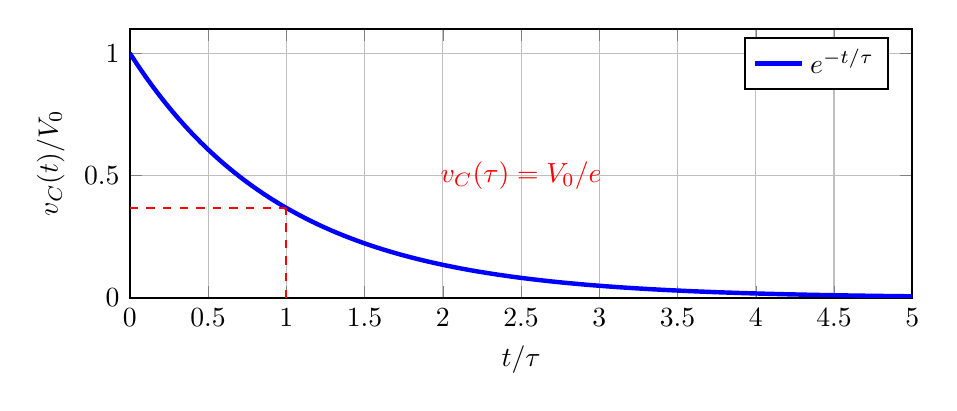
\begin{tikzpicture}
            \begin{axis}[
                width=0.95\textwidth,
                height=5cm,
                xlabel={$t/\tau$},
                ylabel={$v_C(t)/V_0$},
                xmin=0, xmax=5,
                ymin=0, ymax=1.1,
                grid=major,
                legend pos=north east,
                thick
            ]
            \addplot[blue, ultra thick, domain=0:5, samples=100] {exp(-x)};
            \addlegendentry{$e^{-t/\tau}$}
            
            % Mark tau
            \draw[dashed, red] (axis cs: 1,0) -- (axis cs:1,0.368);
            \draw[dashed, red] (axis cs:0,0.368) -- (axis cs:1,0.368);
            \node[red] at (axis cs: 2.5,0.5) {$v_C(\tau) = V_0/e$};
            \end{axis}
        \end{tikzpicture}
        \end{figure}
        
    \end{columns}
    
\end{frame}

\begin{frame}{RC Circuit: Step Response}
    
    \begin{columns}[t]
    \column{0.48\textwidth}
        \textbf{Circuit with DC Source}: 
        
        \begin{figure}[htb]
        \centering
        \begin{circuitikz}[scale=1.0]
            \draw (0,2.5) to[V, l_=$V_s$] (0,0);
            \draw (0,2.5) -- (0.5,2.5);
            \draw (0.5,2.5) -- (1,2.8);
            \draw (1,2.5) -- (1.5,2.5);
            \draw (1.5,2.5) to[R, l=$R$] (3,2.5);
            \draw (3,2.5) to[C, l_=$C$, v^=$v_C$] (3,0);
            \draw (3,0) to[short] (0,0);
            \node at (0.75,3.1) {$t=0$};
            % Arrow indicating switch closing
            \draw[->, thick, red] (1,2.9) -- (1,2.55);
        \end{circuitikz}
        \end{figure}
        
        \textbf{KVL for $t > 0$} and $v_C(0^-) = 0$: 
        \[
        V_s = v_R + v_C = iR + v_C
        \]
        \[
        V_s = RC\frac{dv_C}{dt} + v_C
        \]
        
    \column{0.48\textwidth}
        \textbf{Solution Form}:  
        \[
        v_C(t) = v_C(\infty) + [v_C(0^+) - v_C(\infty)]e^{-t/\tau}
        \]
        
        where: 
        \begin{itemize}
            \item $v_C(0^+) = 0$ (voltage continuity)
            \item $v_C(\infty) = V_s$ (steady-state voltage)
            \item $\tau = RC$
        \end{itemize}
        
        \begin{block}{Step Response}
            \[
            v_C(t) = V_s(1 - e^{-t/RC})
            \]
            \[
            i(t) = \frac{V_s}{R}e^{-t/RC}
            \]
        \end{block}
        
    \end{columns}
    
\end{frame}

\begin{frame}{RC Step Response: Charging Behavior}
    
    \begin{columns}[t]
    \column{0.48\textwidth}
        \textbf{Voltage rises logarithmically}:
        
        \begin{figure}[htb]
        \centering
        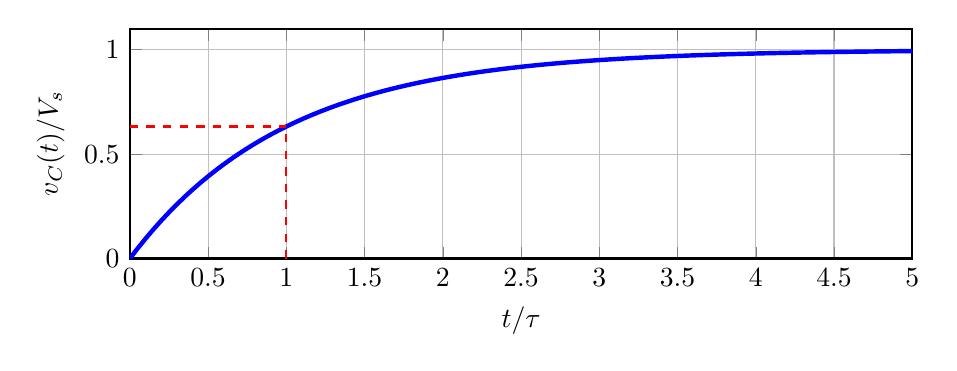
\begin{tikzpicture}
            \begin{axis}[
                width=0.95\textwidth,
                height=4.5cm,
                xlabel={$t/\tau$},
                ylabel={$v_C(t)/V_s$},
                xmin=0, xmax=5,
                ymin=0, ymax=1.1,
                grid=major,
                thick
            ]
            \addplot[blue, ultra thick, domain=0:5, samples=100] {1 - exp(-x)};
            
            % Mark tau
            \draw[dashed, red] (axis cs:1,0) -- (axis cs:1,0.632);
            \draw[dashed, red] (axis cs:0,0.632) -- (axis cs:1,0.632);
            \end{axis}
        \end{tikzpicture}
        \caption{Capacitor voltage}
        \end{figure}
        
    \column{0.48\textwidth}
        \textbf{Current decays exponentially}:
        
        \begin{figure}[htb]
        \centering
        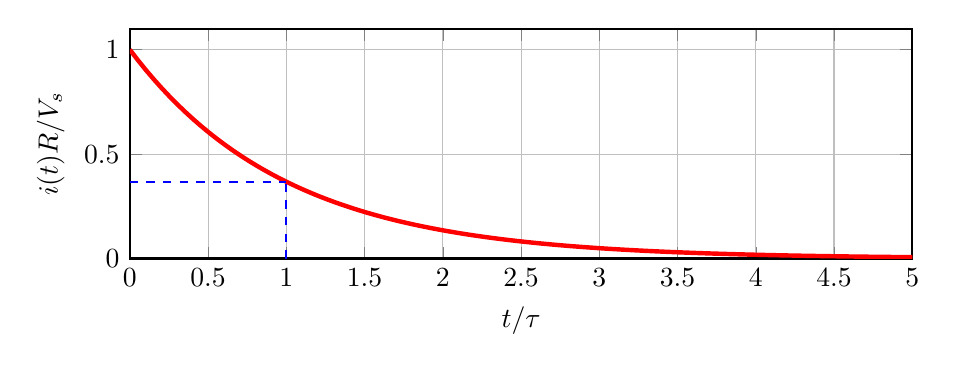
\begin{tikzpicture}
            \begin{axis}[
                width=0.95\textwidth,
                height=4.5cm,
                xlabel={$t/\tau$},
                ylabel={$i(t)R/V_s$},
                xmin=0, xmax=5,
                ymin=0, ymax=1.1,
                grid=major,
                thick
            ]
            \addplot[red, ultra thick, domain=0:5, samples=100] {exp(-x)};
            
            % Mark tau
            \draw[dashed, blue] (axis cs:1,0) -- (axis cs:1,0.368);
            \draw[dashed, blue] (axis cs:0,0.368) -- (axis cs:1,0.368);
            \end{axis}
        \end{tikzpicture}
        \caption{Capacitor current}
        \end{figure}
        
    \end{columns}

    \vspace{-1cm}
    
    \begin{block}{Physical Interpretation}
        Initially:  capacitor is a short circuit ($v_C = 0$, $i$ is maximum)\\
        Finally: capacitor is an open circuit ($v_C = V_s$, $i = 0$)
    \end{block}
    
\end{frame}

\begin{frame}{RL Circuit Analysis: Source-Free Response}
    
    \begin{columns}[t]
    \column{0.48\textwidth}
        \textbf{Circuit}:
        
        \begin{figure}[htb]
        \centering
        \begin{circuitikz}[scale=1.1]
            \draw (0,0) to[L, l=$L$, i^=$i_L$] (0,2);
            \draw (0,2) -- (0.5,2);
            \draw (0.5,2) -- (1,2.3);
            \draw (1,2) -- (2,2);
            \draw (2,2) to[R, l=$R$] (2,0);
            \draw (2,0) to[short] (0,0);
            \node at (0.75,2.6) {$t=0$};
            % Arrow indicating switch closing
            \draw[->, thick, red] (1,2.4) -- (1,2.05);
        \end{circuitikz}
        \end{figure}
        
        \textbf{Initial Condition}: $i_L(0) = I_0$
        
        \textbf{Apply KVL}: 
        \[
        v_L + v_R = 0
        \]
        \[
        L\frac{di_L}{dt} + Ri_L = 0
        \]
        
    \column{0.48\textwidth}
        \textbf{Differential Equation}:
        \[
        \frac{di_L}{dt} + \frac{R}{L}i_L = 0
        \]
        
        \textbf{Solution}:  Assume $i_L(t) = Ke^{st}$
        \[
        s + \frac{R}{L} = 0 \quad \Rightarrow \quad s = -\frac{R}{L}
        \]
        
        \begin{block}{General Solution}
            \[
            i_L(t) = I_0 e^{-Rt/L}
            \]
            \[
            v_L(t) = L\frac{di_L}{dt} = -RI_0 e^{-Rt/L}
            \]
        \end{block}
 
    \end{columns}
    
\end{frame}

\begin{frame}{RL Circuit: Step Response}
    
    \begin{columns}[t]
    \column{0.48\textwidth}
        \textbf{Circuit with DC Source}:
        
        \begin{figure}[htb]
        \centering
        \begin{circuitikz}[scale=1.0]
            \draw (0,2.5) to[V, l_=$V_s$] (0,0);
            \draw (0,2.5) -- (0.5,2.5);
            \draw (0.5,2.5) -- (1,2.8);
            \draw (1,2.5) -- (1.5,2.5);
            \draw (1.5,2.5) to[R, l=$R$] (3,2.5);
            \draw (3,2.5) to[L, l=$L$, i^=$i_L$] (3,0);
            \draw (3,0) to[short] (0,0);
            \node at (0.75,3.1) {$t=0$};
            % Arrow indicating switch closing
            \draw[->, thick, red] (1,2.9) -- (1,2.55);
        \end{circuitikz}
        \end{figure}
        
        \textbf{Initial Condition}: $i_L(0^-) = 0$
        
        \vspace{0.3cm}
        
        \textbf{KVL for $t > 0$}: 
        \[
        V_s = v_R + v_L = Ri_L + L\frac{di_L}{dt}
        \]
        
    \column{0.48\textwidth}
        \textbf{Solution Form}:  
        \[
        i_L(t) = i_L(\infty) + [i_L(0^+) - i_L(\infty)]e^{-t/\tau}
        \]
        
        where: 
        \begin{itemize}
            \item $i_L(0^+) = 0$ (currrent continuity)
            \item $i_L(\infty) = V_s/R$ (current steady-state)
            \item $\tau = L/R$
        \end{itemize}
        
        \begin{block}{Step Response}
            \[
            i_L(t) = \frac{V_s}{R}(1 - e^{-Rt/L})
            \]       
            \[
            v_L(t) = V_s e^{-Rt/L}
            \]
        \end{block}
        
    \end{columns}
    
\end{frame}

\begin{frame}{General Solution Method for First-Order Circuits}
    
    \begin{enumerate}
        \item \textbf{Find Initial Condition}:  $x(0^+)$
        \begin{itemize}
            \item Use continuity: $v_C(0^+) = v_C(0^-)$ or $i_L(0^+) = i_L(0^-)$
            \item Analyze circuit just before switching occurs
        \end{itemize}
        
        \item \textbf{Find Final (Steady-State) Value}: $x(\infty)$
        \begin{itemize}
            \item Capacitors become open circuits (DC)
            \item Inductors become short circuits (DC)
            \item Solve the DC circuit
        \end{itemize}
        
        \item \textbf{Find Time Constant}: $\tau$
        \begin{itemize}
            \item RC circuits: $\tau = R_{\text{eq}}C$
            \item RL circuits: $\tau = L/R_{\text{eq}}$
            \item $R_{\text{eq}}$ is Th\'evenin resistance seen by L or C
        \end{itemize}
    \end{enumerate}
    
    \begin{block}{General Solution}
        \[
        x(t) = x(\infty) + [x(0^+) - x(\infty)]e^{-t/\tau}
        \]
    \end{block}
    
\end{frame}

\section{Second-Order Circuits}

\begin{frame}{Second-Order Circuits: RLC Combinations}
    
    \begin{columns}[t]
    \column{0.48\textwidth}
        \textbf{What is a Second-Order Circuit? }
        
        \vspace{0.3cm}
        
        A circuit containing: 
        \begin{itemize}
            \item \textbf{Two} energy storage elements
            \item Energy storage devices may be L or C
            \item Resistors and sources
        \end{itemize}
        
        \vspace{0.5cm}
        
        \begin{block}{Mathematical Form}
            Results in a \textbf{second-order} differential equation: 
            \[
            \frac{d^2x}{dt^2} + 2\alpha\frac{dx}{dt} + \omega_0^2 x = f(t)
            \]
        \end{block}
        
    \column{0.48\textwidth}
        
        \begin{figure}[htb]
        \centering
        \begin{circuitikz}[scale=0.75]
            \draw (0,3) to[V, l_=$V_s$] (0,0);
            \draw (0,3) -- (0.35,3);
            \draw (0.35,3) -- (0.7,3.25);
            \draw (0.7,3) -- (1,3);
            \draw (1,3) to[R, l=$R$] (2.5,3);
            \draw (2.5,3) to[L, l=$L$] (4,3);
            \draw (4,3) to[C, l=$C$] (4,0);
            \draw (4,0) to[short] (0,0);
            \node at (0.5,3.55) {$t=0$};
            % Arrow indicating switch closing
            \draw[->, thick, red] (0.7,3.35) -- (0.7,3.05);
        \end{circuitikz}
        \end{figure}

        \begin{figure}[htb]
        \centering
        \begin{circuitikz}[scale=1.0]
            \draw (0,0) to[I, l=$I_s$] (0,2.5);
            \draw (0,2.5) to[short] (1,2.5)
                  to[R, l=$R$] (1,0);
            \draw (1,2.5) to[short] (2,2.5)
                  to[L, l=$L$] (2,0);
            \draw (2,2.5) to[short] (3,2.5)
                  to[C, l=$C$] (3,0);
            \draw (0,0) to[short] (3,0);
        \end{circuitikz}
        \end{figure}
        
    \end{columns}
    
\end{frame}

\begin{frame}{Series RLC Circuit: Differential Equation}
    
    \begin{columns}[t]
    \column{0.48\textwidth}
        \textbf{Source-Free Series RLC}:
        
        \begin{figure}[htb]
        \centering
        \begin{circuitikz}[scale=0.75]
            \draw (0,0) to[R, l=$R$, i=$i$] (0,2.5)
                  to[L, l=$L$] (2.5,2.5)
                  to[C, l_=$C$, v^=$v_C$] (2.5,0) -- (0,0);
        \end{circuitikz}
        \end{figure}
        
        \[
        v_R + v_L + v_C = 0
        \]
        \[
        Ri + L\frac{di}{dt} + v_C = 0
        \]
        \[
        RC\frac{dv_C}{dt} + LC\frac{d^2v_C}{dt^2} + v_C = 0
        \]
        
    \column{0.48\textwidth}
        \textbf{Standard Form}:
        \[
        \frac{d^2v_C}{dt^2} + \frac{R}{L}\frac{dv_C}{dt} + \frac{1}{LC}v_C = 0
        \]

        \vspace{0.5cm}

        Natural Frequency: $\omega_0 = \frac{1}{\sqrt{LC}}$

        \vspace{0.1cm}

        Damping Coefficient: $\alpha = \frac{R}{2L}$

        \vspace{0.2cm}
        
        \begin{block}{Standard Form}
            \[
            \frac{d^2v_C}{dt^2} + 2\alpha\frac{dv_C}{dt} + \omega_0^2 v_C = 0
            \]
        \end{block}
        
    \end{columns}
    
\end{frame}

\begin{frame}{Characteristic Equation and Damping}
    
    \begin{columns}[t]
    \column{0.48\textwidth}
        \textbf{Characteristic Equation}:
        
        Assume solution: $v_C(t) = Ke^{st}$
        \[
        s^2 + 2\alpha s + \omega_0^2 = 0
        \]
        
        \textbf{Roots}:
        \[
        s_{1,2} = -\alpha \pm \sqrt{\alpha^2 - \omega_0^2}
        \]
        
        \vspace{0.3cm}
        
        \textbf{Damping Ratio}:
        \[
        \zeta = \frac{\alpha}{\omega_0} = \frac{R}{2}\sqrt{\frac{C}{L}}
        \]
        
    \column{0.48\textwidth}
        \textbf{Three Cases}:
        
        \vspace{0.3cm}
        
        \begin{enumerate}
            \item \textbf{Overdamped}:  $\alpha > \omega_0$ ($\zeta > 1$)
            \begin{itemize}
                \item Two real, distinct roots
                \item No oscillation
            \end{itemize}
            
            \vspace{0.2cm}
            
            \item \textbf{Critically Damped}: $\alpha = \omega_0$ ($\zeta = 1$)
            \begin{itemize}
                \item Two real, equal roots
                \item Fastest response without overshoot
            \end{itemize}
            
            \vspace{0.2cm}
            
            \item \textbf{Underdamped}: $\alpha < \omega_0$ ($\zeta < 1$)
            \begin{itemize}
                \item Complex conjugate roots
                \item Oscillatory response
            \end{itemize}
        \end{enumerate}
        
    \end{columns}
    
\end{frame}

\begin{frame}{Overdamped Response ($\alpha > \omega_0$)}
    
    \begin{columns}[t]
    \column{0.48\textwidth}
        \textbf{Roots}:
        \[
        s_1 = -\alpha + \sqrt{\alpha^2 - \omega_0^2}
        \]
        \[
        s_2 = -\alpha - \sqrt{\alpha^2 - \omega_0^2}
        \]
        
        Both roots are \textbf{real and negative}.
        
        \vspace{0.5cm}
        
        \begin{block}{General Solution}
            \[
            v_C(t) = A_1 e^{s_1 t} + A_2 e^{s_2 t}
            \]
            where $A_1$ and $A_2$ are determined by initial conditions
        \end{block}
        
    \column{0.48\textwidth}
        \textbf{Response Shape}:
        
        \begin{figure}[htb]
        \centering
        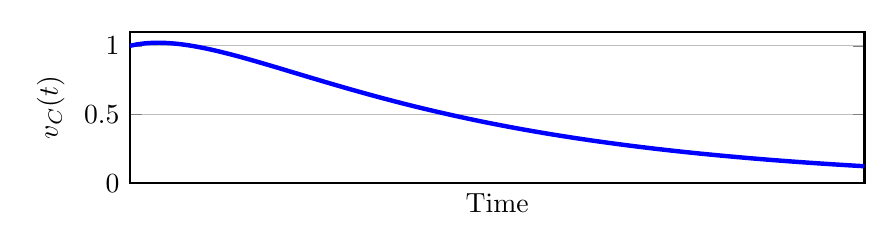
\begin{tikzpicture}
            \begin{axis}[
                width=0.9\textwidth,
                height=3.5cm,
                xlabel={Time},
                ylabel={$v_C(t)$},
                xmin=0, xmax=5,
                ymin=0, ymax=1.1,
                grid=major,
                thick,
                ytick={0, 0.5, 1},
                xtick=\empty
            ]
            % Overdamped response
            \addplot[blue, ultra thick, domain=0:5, samples=100] 
                {1.5*exp(-0.5*x) - 0.5*exp(-2*x)};
            \end{axis}
        \end{tikzpicture}
        \caption{Slow exponential decay, no oscillation}
        \end{figure}
        
        \vspace{0.3cm}
        
        \textbf{Characteristics}:
        \begin{itemize}
            \item No overshoot
            \item Slow settling
            \item High resistance
        \end{itemize}
        
    \end{columns}
    
\end{frame}

\begin{frame}{Critically Damped Response ($\alpha = \omega_0$)}
    
    \begin{columns}[t]
    \column{0.48\textwidth}
        \textbf{Roots}: 
        \[
        s_1 = s_2 = -\alpha
        \]
        
        Repeated real root.
        
        \vspace{0.5cm}
        
        \begin{block}{General Solution}
            \[
            v_C(t) = (A_1 + A_2 t) e^{-\alpha t}
            \]
            where $A_1$ and $A_2$ are determined by initial conditions
        \end{block}
        
        \vspace{0.3cm}
        
        \textbf{Critical Resistance}:
        \[
        R_{\text{crit}} = 2\sqrt{\frac{L}{C}}
        \]
        
    \column{0.48\textwidth}
        \textbf{Response Shape}:
        
        \begin{figure}[htb]
        \centering
        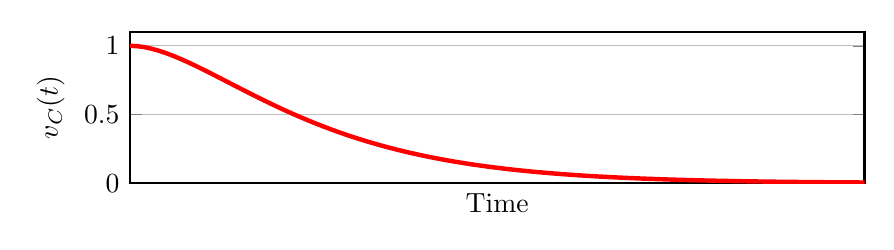
\begin{tikzpicture}
            \begin{axis}[
                width=0.9\textwidth,
                height=3.5cm,
                xlabel={Time},
                ylabel={$v_C(t)$},
                xmin=0, xmax=5,
                ymin=0, ymax=1.1,
                grid=major,
                thick,
                ytick={0, 0.5, 1},
                xtick=\empty
            ]
            % Critically damped
            \addplot[red, ultra thick, domain=0:5, samples=100] 
                {(1 + 1.5*x)*exp(-1.5*x)};
            \end{axis}
        \end{tikzpicture}
        \caption{Fastest settling without overshoot}
        \end{figure}
        
        \vspace{0.3cm}
        
        \textbf{Characteristics}:
        \begin{itemize}
            \item No overshoot
            \item Fastest response
            \item Boundary case
        \end{itemize}
        
    \end{columns}
    
\end{frame}

\begin{frame}{Underdamped Response ($\alpha < \omega_0$)}
    
    \begin{columns}[t]
    \column{0.48\textwidth}
        \textbf{Roots}:
        \[
        s_{1,2} = -\alpha \pm j\omega_d
        \]
        
        where the \textbf{damped frequency} is: 
        \[
        \omega_d = \sqrt{\omega_0^2 - \alpha^2}
        \]
        
        \vspace{-0.3cm}
        
        \begin{block}{General Solution}
            \[
            v_C(t) = e^{-\alpha t}(A_1 \cos(\omega_d t) + A_2 \sin(\omega_d t))
            \]
            or equivalently:
            \[
            v_C(t) = B e^{-\alpha t} \cos(\omega_d t + \phi)
            \]
        \end{block}
        
    \column{0.48\textwidth}
        \textbf{Response Shape}:
        
        \begin{figure}[htb]
        \centering
        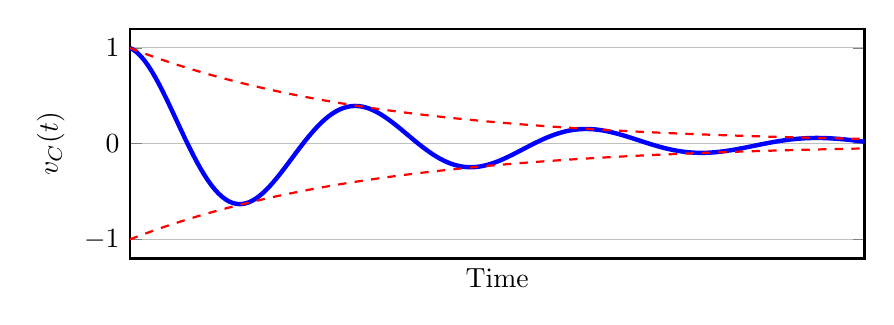
\begin{tikzpicture}
            \begin{axis}[
                width=0.9\textwidth,
                height=4.5cm,
                xlabel={Time},
                ylabel={$v_C(t)$},
                xmin=0, xmax=10,
                ymin=-1.2, ymax=1.2,
                grid=major,
                thick,
                xtick=\empty
            ]
            % Underdamped response
            \addplot[blue, ultra thick, domain=0:10, samples=200] 
                {exp(-0.3*x)*cos(deg(2*x))};
            % Envelope
            \addplot[red, dashed, domain=0:10, samples=100] 
                {exp(-0.3*x)};
            \addplot[red, dashed, domain=0:10, samples=100] 
                {-exp(-0.3*x)};
            \end{axis}
        \end{tikzpicture}
        \caption{Oscillatory with exponential decay}
        \end{figure}
        
        \textbf{Characteristics}: 
        \begin{itemize}
            \item Oscillates at $\omega_d$
            \item Envelope decays at rate $\alpha$
            \item Low resistance
        \end{itemize}
        
    \end{columns}
    
\end{frame}

\begin{frame}{Comparison of Damping Cases}
    
    \begin{figure}[htb]
    \centering
    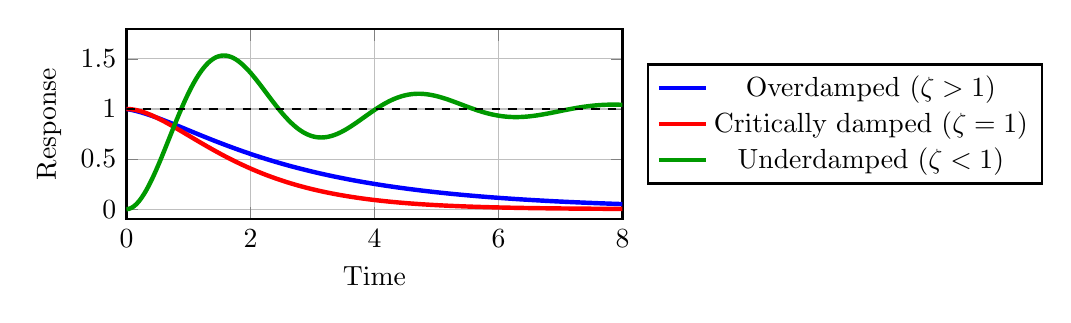
\begin{tikzpicture}
        \begin{axis}[
            width=0.65\textwidth,
            height=4cm,
            xlabel={Time},
            ylabel={Response},
            xmin=0, xmax=8,
            ymin=-0.1, ymax=1.8,
            grid=major,
            legend style={at={(1.05,0.5)}, anchor=west},
            thick
        ]
        % Overdamped
        \addplot[blue, ultra thick, domain=0:8, samples=100] 
            {1.25*exp(-0.4*x) - 0.25*exp(-1.6*x)};
        \addlegendentry{Overdamped ($\zeta > 1$)}
        
        % Critically damped
        \addplot[red, ultra thick, domain=0:8, samples=100] 
            {(1 + x)*exp(-x)};
        \addlegendentry{Critically damped ($\zeta = 1$)}
        
        % Underdamped
        \addplot[green! 60! black, ultra thick, domain=0:8, samples=200] 
            {1 - exp(-0.4*x)*cos(deg(2*x)) - 0.2*exp(-0.4*x)*sin(deg(2*x))};
        \addlegendentry{Underdamped ($\zeta < 1$)}
        
        % Target line
        \addplot[black, dashed, domain=0:8] {1};
        \end{axis}
    \end{tikzpicture}
    \end{figure}
    
    \begin{block}{Design Implications}
        \begin{itemize}
            \item \textbf{Overdamped}:  Slow but stable (e.g., door closers)
            \item \textbf{Critically damped}:  Optimal speed without overshoot (e.g., measuring instruments)
            \item \textbf{Underdamped}:  Fast but oscillatory (e.g., speakers, control systems)
        \end{itemize}
    \end{block}
    
\end{frame}

\begin{frame}{Parallel RLC Circuit}
    
    \begin{columns}[t]
    \column{0.48\textwidth}
        \textbf{Source-Free Parallel RLC}: 
        
        \begin{figure}[htb]
        \centering
        \begin{circuitikz}[scale=1.0]
            \draw (0,0) to[R, l=$R$] (0,2.5);
            \draw (0,2.5) to[short] (1.5,2.5)
                  to[L, l=$L$, i=$i_L$] (1.5,0);
            \draw (1.5,2.5) to[short] (3,2.5)
                  to[C, l=$C$] (3,0);
            \draw (0,0) to[short] (3,0);
            \node[above] at (1.5,2.5) {$v$};
        \end{circuitikz}
        \end{figure}
        
        \textbf{Apply KCL}:
        \[
        i_R + i_L + i_C = 0
        \]
        \[
        \frac{v}{R} + \frac{1}{L}\int v \, dt + C\frac{dv}{dt} = 0
        \]
        
    \column{0.48\textwidth}
        \textbf{Differentiate and rearrange}:
        \[
        \frac{d^2v}{dt^2} + \frac{1}{RC}\frac{dv}{dt} + \frac{1}{LC}v = 0
        \]

        \vspace{0.5cm}

        Natural Frequency: $\omega_0 = \frac{1}{\sqrt{LC}}$

        \vspace{0.1cm}

        Damping Coefficient: $\alpha = \frac{1}{2RC}$

        \vspace{1cm}
        
        \textbf{Note}:  Same $\omega_0$ as series RLC, but damping depends on $1/R$ (opposite of series)
        
    \end{columns}
    
\end{frame}

\section{Summary}

\begin{frame}{Summary:  Time Domain Analysis}
    
    \begin{columns}[t]
    \column{0.48\textwidth}
        \textbf{First-Order Circuits}:
        \begin{itemize}
            \item One energy storage element (L or C)
            \item First-order differential equation
            \item Exponential response:  $e^{-t/\tau}$
            \item Time constant: $\tau = RC$ or $\tau = L/R$
        \end{itemize}
        
        \textbf{Solution Method}:
        \[
        x(t) = x(\infty) + [x(0^+) - x(\infty)]e^{-t/\tau}
        \]
        
        \textbf{Key Concepts}:
        \begin{itemize}
            \item Continuity of $v_C$ and $i_L$
            \item Initial conditions
            \item Steady-state values
        \end{itemize}
        
    \column{0.48\textwidth}
        \textbf{Second-Order Circuits}:
        \begin{itemize}
            \item Two energy storage elements
            \item Second-order differential equation
            \item Response depends on damping
        \end{itemize}
        
        % \vspace{0.3cm}
        
        \textbf{Damping Cases}:
        \begin{enumerate}
            \item Overdamped: slow, no oscillation
            \item Critically damped: fastest, no overshoot
            \item Underdamped: oscillatory
        \end{enumerate}
        
        % \vspace{0.3cm}
        
        \textbf{Parameters}:
        \begin{itemize}
            \item Natural frequency: $\omega_0 = 1/\sqrt{LC}$
            \item Damping coefficient: $\alpha$
            \item Damping ratio: $\zeta = \alpha/\omega_0$
        \end{itemize}
        
    \end{columns}
    
\end{frame}

\end{document}